\section{Performance Evaluation}
\label{sec:expr}

\begin{table}[!t]
	%\vspace{-0.1in}
	\caption{Parameter of RealWorld Graph }
	\hspace{-0.15in}
	\vspace{0.0in}
	\label{tab:Dataset}
	\centering
	\small
	\begin{tabular}{c|c|c|c}
		\hline\hline
		{\textbf{Name}} &
		{\textbf{Vertices}} &
		{\textbf{Edges}} &
		{\textbf{Source}} \\
		\hline
		{\textbf{Flickr}} & 2,302,925 &33,140,017   & \cite{mislove-2008-flickr}\\
		\hline
		{\textbf{LiveJournal}} & 4,847,571 & 68,475,391 &\cite{livejournal}\\
		\hline
		{\textbf{Orkut}} &3,072,441& 117,184,899 & \cite{mislove-2007-socialnetworks} \\
		\hline
		{\textbf{culeweb09}} & 20,000,000 & 243,063,334 &\cite{clueweb}\\		\hline
		{\textbf{Wiki-link}} & 12,150,976 &378,142,420&\cite{wikilinks} \\
		\hline
		{\textbf{arabic-2005}} & 22,744,080 & 639,999,458 &\cite{arabic-2005}\\		\hline
		\hline
	\end{tabular}
	\vspace{-0.1in}
	
\end{table}
\Paragraph{Experimental Setup and Datasets.}
Our experiments are conducted on 16 node Aliyun ECS cluster(ecs.r5.xlarge), each runs Ubuntu 16.04 LTS and has 4 vCPUs and 32GB memory. The network bandwidth between instance workers is 1.5Gbps/s. And all the works uses Hadoop 2.6.4 as distributed file system.

Table \ref{tab:Dataset} shows the real world graphs used for all graph algorithm, And to we syntheticly generate several tree structure Datasets with 128000000 Node and  ** edges. 

We compare A3log with three state-of-the-art Datalog frameworks. \textbf{SociaLite} \cite{Lam:2013:SDE:2510649.2511289,Seo:2013:DSD:2556549.2556572} is a Datalog implementation for social network analysis. \textbf{Myria} \cite{Halperin:2014:DMB:2588555.2594530,Wang:2015:AFR:2824032.2824052} supports Datalog asynchronous evaluation. And \textbf{BigDatalog}\cite{Shkapsky:2016:BDA:2882903.2915229} a Datalog implementation based on spark. All these three framework support monotonic aggregation inside recursion.


\subsection{Comparison to Other Systems}




For each system, one instance was dedicated as the master and each of the 15 worker nodes was allowed 30GB memory and 4 threads, Myria was configured with one instance of Myria and PostgreSQL per node. Bigdatalog was configured with Single-Job PSN with SetRDD and 60 for shuffle partition. And we configure the asynchronous A3log with adaptive message buffer strategy to obtain asynchronous result. The runtime results are the execution time excluding data loading time, and each is a mean of three runs.

We compare A3Log with other systems in the context of three algorithms, SSSP, Connected Components(Asynchronizable) and PageRank(convertible). These three algorithms are all supported by these systems except PagreRank\footnote{Since BigDatalog doesn't support monotonic aggregate function $msum$ and $mcount$, so it is hard to express PageRank computation with BigDatalog. So we use GraphX as a instead for PageRank experiment.}. Figure \ref{fig:dist-result} shows the experimental result for system comparision. 

\textbf{CC} Connected component program is a label propagation approach for determining the lowest vertex id a vertex is connected to. The aggregate operation is $\$min$ and the nonaggregate operation satisfy the accumulable conditions, which can be asynchronized directly. As reported in Figures \ref{fig:dist-result}(a), asynchronous A3log consistently outperform all these three competitor. Only Socialite beats the synchronous version A3log on Orkut datasets\footnote{Socialite has run out of memory on wiki-link datasets.}. 

\textbf{SSSP} Single source shortest path is another Asynchronus Algorithm. As reported in Figures \ref{fig:dist-result}(b), asynchronous A3log outperforms all these three competior. But asynchronous A3log doesn't beat synchronous A3log on Flickr and LiveJournal the two relatively small datasets, But the later experiments show that our optimization technology performs quite well on big datasets.

\textbf{PageRank} PageRank algorithm, is a link analysis algorithm for web searching which computes the importance of node in a graph. The aggregate operator is $\$sum$ which does not satisfy the acccumulable conditions, but it can be  asynchronized by section \ref{coro:auto:2}. As reported in Figures \ref{fig:dist-result}(c), Synchronous A3log outperforms all the other system except Bigdatalog/GraphX on Orkut dataset. The asynchronous A3log consistently outperforms the other systems and also synchronous processing. The synchronous A3log is slower than Bigdatalog only on Orkut. And Socialite is no longer competitive without the support of seminaive technology.

\subsection{Effectiveness of Adaptive Message Buffer}
\label{sec:expr:AMBuffer}
\begin{figure*}[!t]
	\vspace{0.0in}
	\centering
	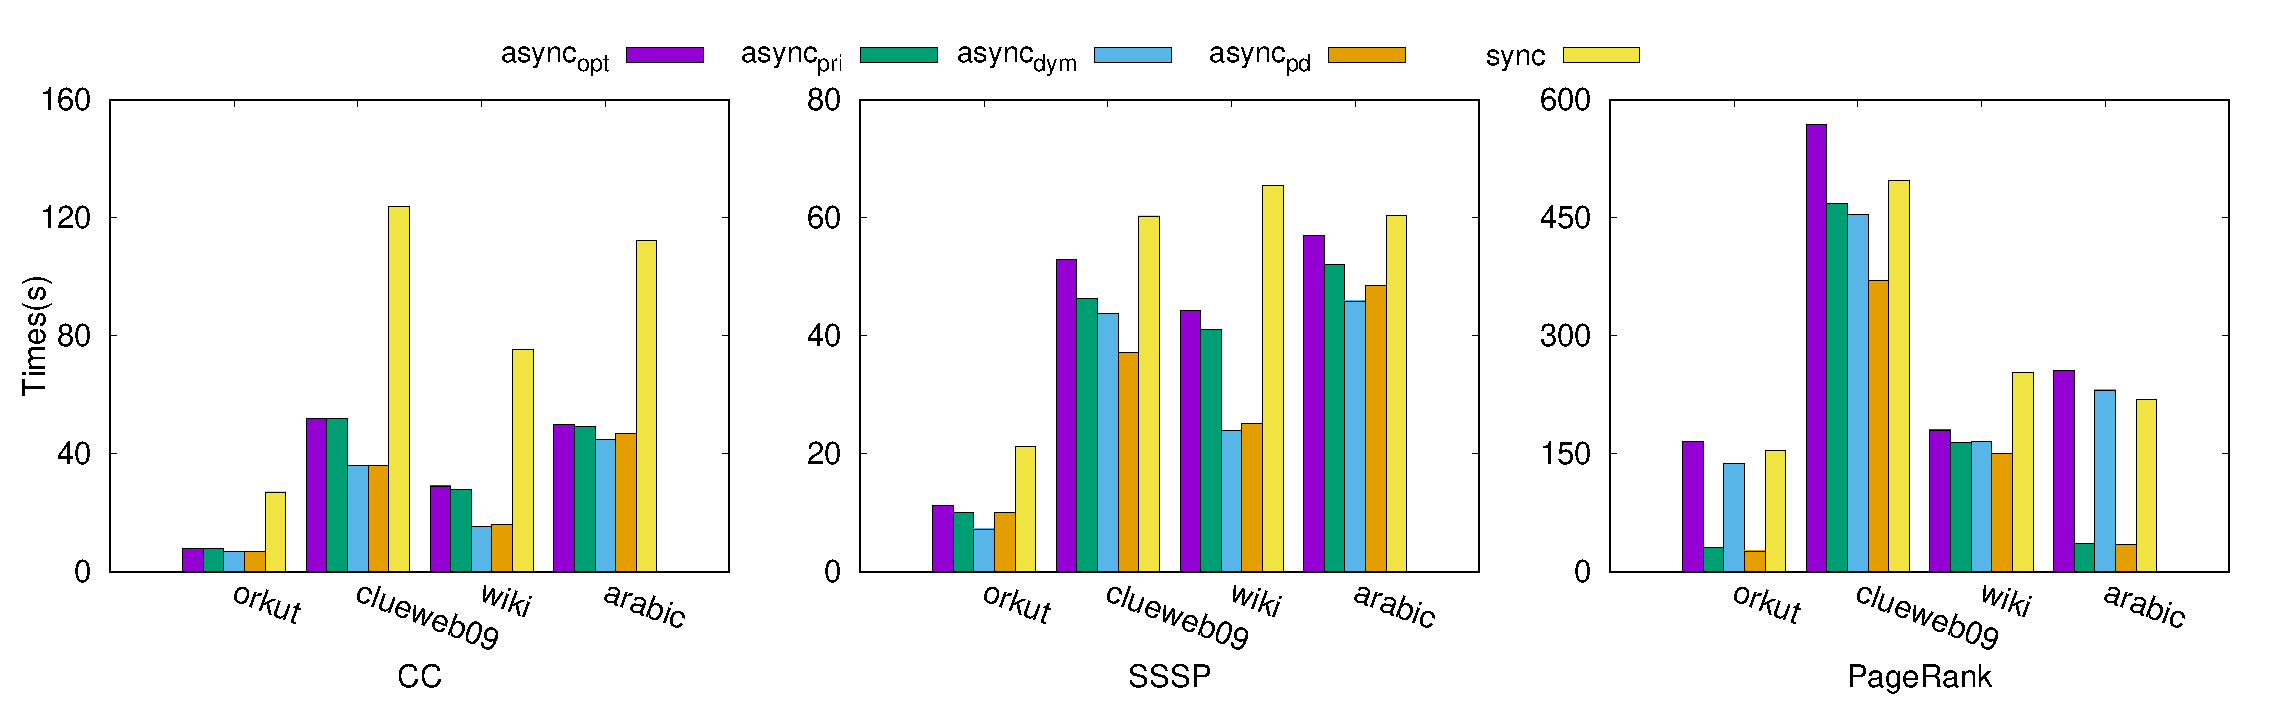
\includegraphics[width=7.0in]{figuration/summary.eps}
	\vspace{-0.1in}
	\caption{Effectiveness of Adaptive Message Buffer}
	\label{fig:summary}
	\vspace{-0.1in}
\end{figure*}
\begin{figure*}[!t]
	\centering
	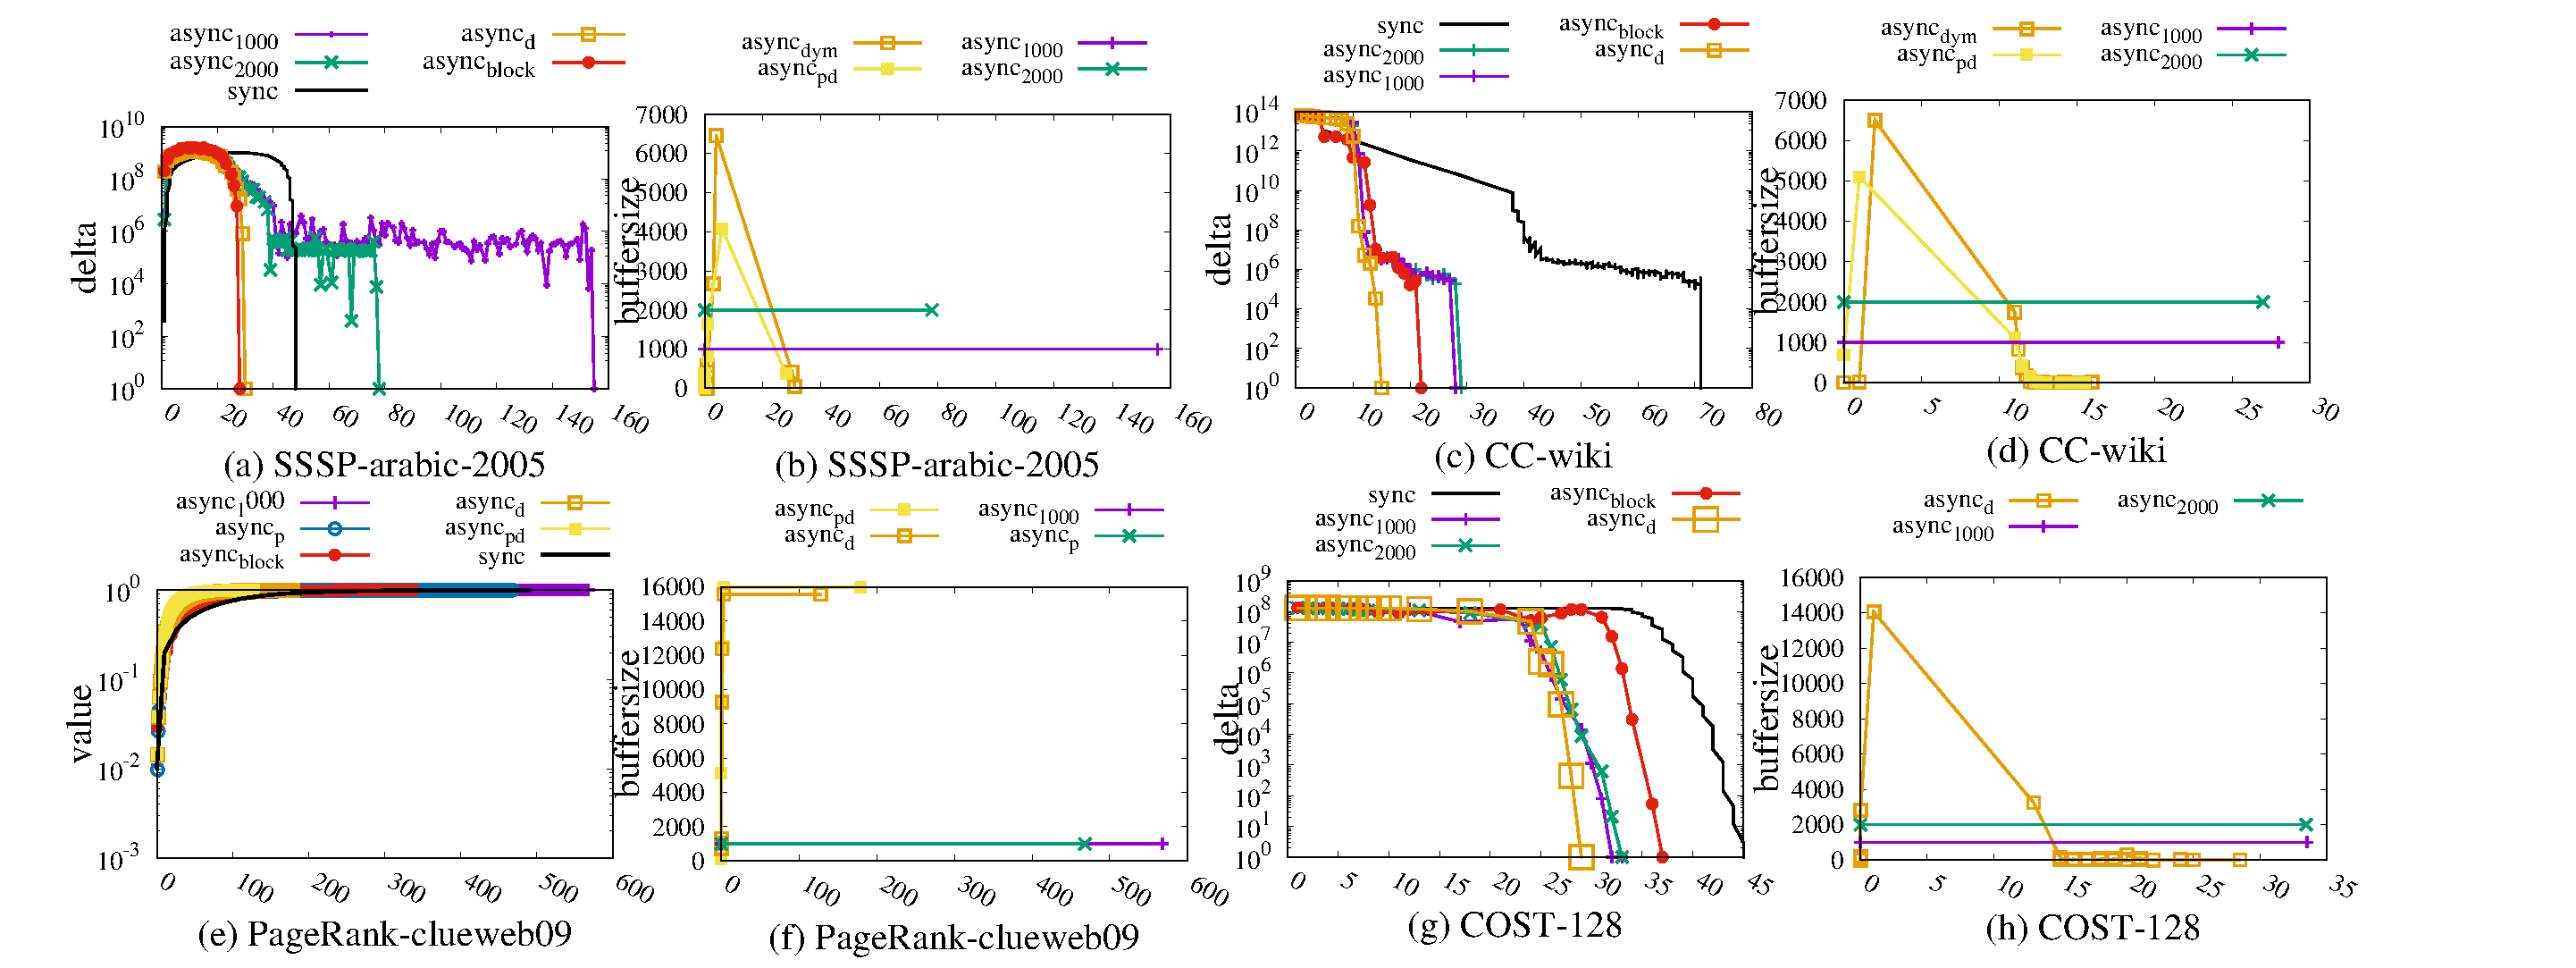
\includegraphics[width=7.0in]{figuration/combine.eps}
	\vspace{-0.1in}
	\caption{Effectiveness of Adaptive Message Buffer}
	\label{fig:details}
	\vspace{-0.1in}
\end{figure*}



In this section, we evaluate the effeiciency of adaptive message buffer strategy described in \ref{} with four application \texttt{CC}, \texttt{SSSP}, \texttt{PageRank} and \texttt{What is the cost of each part}\cite{7113340} a n algorithm commonly used in cost estimation. And for the \textbf{COST} algorithm we synthetically generate a hierarchical (tree-like) dataset with 128000000 tree nodes.

We compared the performance of adaptive message buffer startegy(denote by Async${amb}$) with (1) Synchronous processing, (2) Asynchronous processing with fixed buffersize (Vertex-centric), (3) Asynchronous processing with fixed buffer size and priority scheduling and (4) Block-centric processing, denoted by Sync, Async$_{fix}$, Async$_{pri}$ and Async$_{block}$. Further we also performed asynchronous processing with both adaptive buffer size and priority scheduling, denote by Async$_{ambp}$. Since determine the optimal message buffer size of Async$_{fix}$ is quite hard, so we fixed the buffersize to 500, 1000 and 2000 in turn, and choose the best one as result.


\Paragraph{CC} Figure \ref{fig:summary}(a) report the performance of CC algorithm. Async$_amb$ consistently outperform all these cases. Over clueweb09 (resp. wiki and arabic-2005), it is on average 3.63(resp. 4.89 and 1.34) times, 1.24(resp. 1.82 and 4.44) times and  2.61(resp. 1.50, 1.08) times faster than that of \textbf{Sync}, Async$_{fix}$, Async$_{block}$, respectively. 

\textcolor{blue}{
The performance gain of Async${amb}$ comes from the following:
(1) reduction of invalid computation and communication latency by the use of adaptive message buffer strategy; 
(2) the semi-naive evaluation technology;
(3) ecfficient executing enginee with asynctable for accumulative asynchronous processing.
Note that other strategy can also benefit from (2) and (3)}
For example in Figure \ref{fig:details}(c) and (d) Both async$_{fix}$ and  async$_{block}$ will slow down at the end of the convergence. since the message amount in this stage is drastically reducing. neighter async$_{block}$ nor async$_{fix}$ can perform their best performance. The async$_{amb}$ makes effective use of network strategy by auto tuning message buffer.

\Paragraph{SSSP} Figure \ref{fig:summary}(b) report the performance of SSSP algorithm. Async$_amb$ consistently outperform all these cases except Async$_{block}$ over arabic-2005 datasets. Over clueweb09 (resp. wiki and arabic-2005), it is on average  \textbf{1.60}(resp. 2.74 and 2.02) times, \textbf{1.21}(resp. 1.85 and 5.02) times and  \textbf{1.62}(resp. 1.66 and 0.97) times faster than that of \textbf{Sync}, Async$_{fix}$, Async$_{block}$, respectively. 

As reported in Figure \ref{fig:details}(c) and (d) Async$_{fix}$ shows disastrous performance when little buffer size meet large amount of message. Async$_amb$ doesn't shows no advantage over arabic-2005 because the amount of message doesn't significantly change.


\Paragraph{PageRank} Figure \ref{fig:summary}(c) report the performance of PageRank algorithm. Unlike the other algorithm, The message of Pagerank doesn't not significant changing, so only some buffer sensitive workload (Clueweb09) can benefit from Async$_{amb}$. Howerver PageRank can benefit a lot from Priority scheduling technology, because Async$_pri$ can transmitted larger update in unit message. So we can use a combine strategy i.e., Async$_{ambp}$ strategy, says 3.04,1.73 and 5.36  times faster than that of \textbf{Sync}.
 
{\color{blue} need some experiment
\Paragraph{COST} Cost Algorithm can also benefit a lot from asynchronous processing as shown in figure 
}
 \subsection{Scaling Performance}
 \begin{figure}[!t]
	\vspace{0.1in}
	\centering
	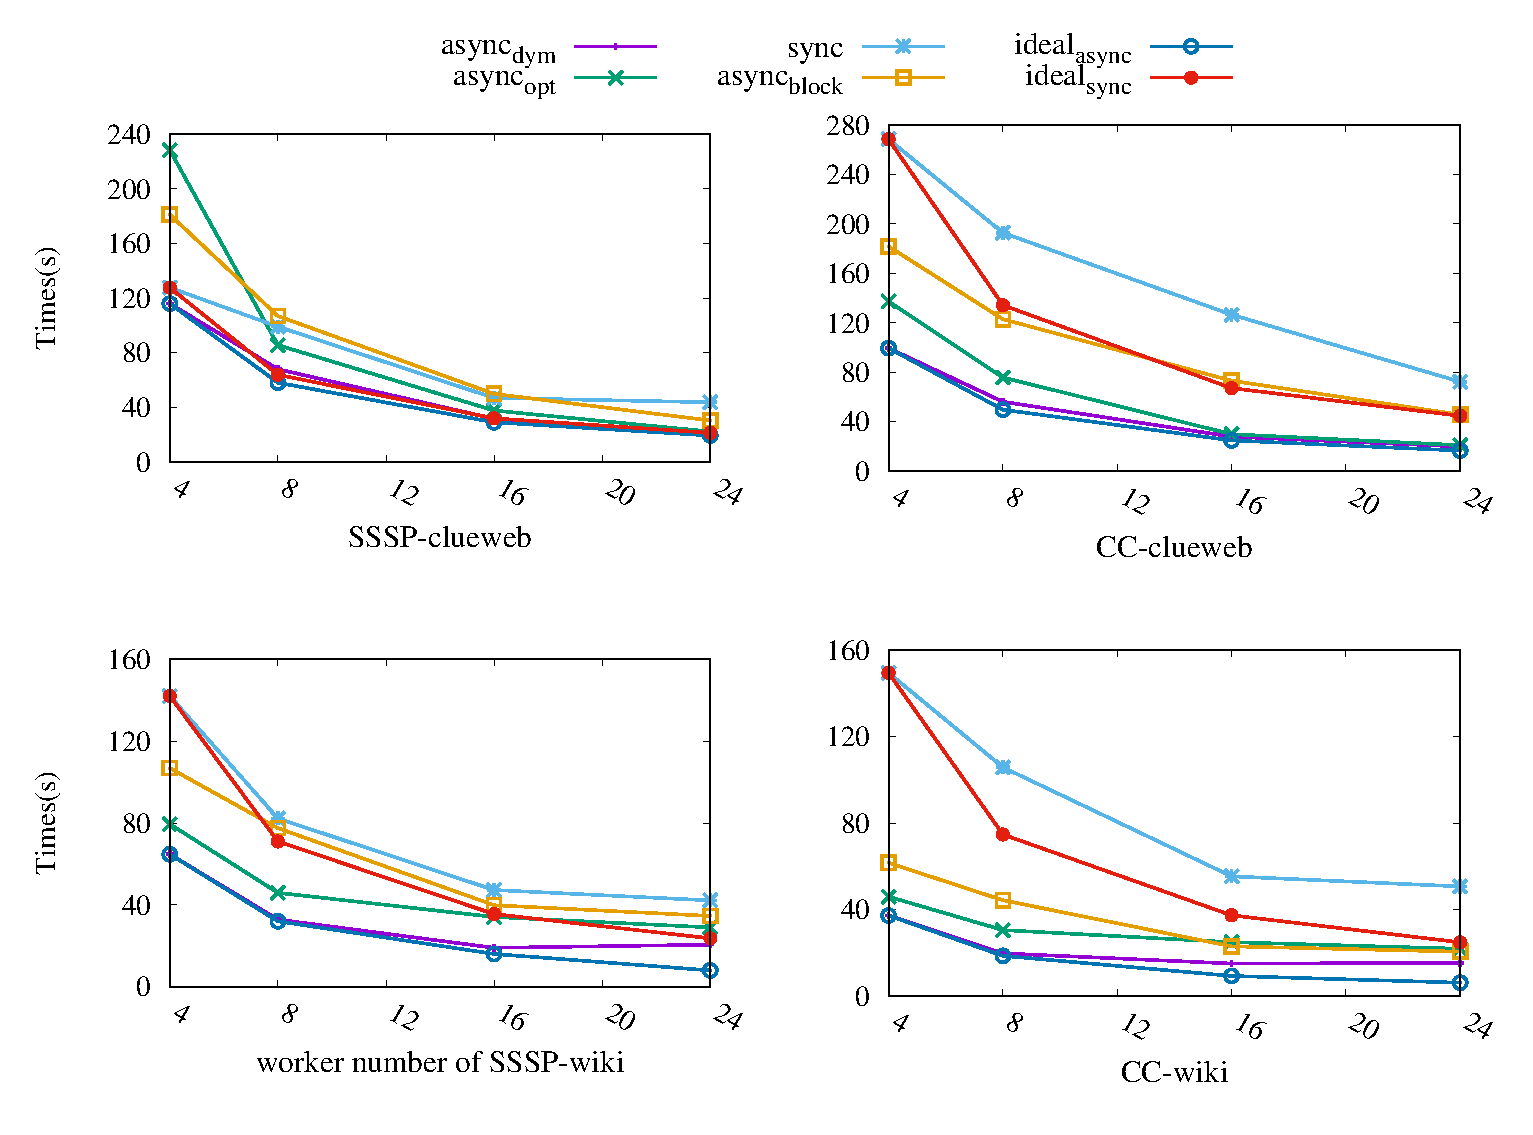
\includegraphics[width=3.4in]{figuration/scale.eps}
	\vspace{-0.1in}
	\caption{Scaling Performance}
	\label{fig:scale}
	\vspace{-0.2in}
\end{figure}

 Here we report more experimental result of how Asynchronous Processing scale over different cluster size. 
 In this set of experiments, we use wiki-link and clueweb09 graphs that can be evaluated on all cluster sizes.
 We compare the scale performance of Async$_{amb}$ with Sync, Async$_{fix}$ and Async$_{block}$. We also draw the ideal scaling performance curve based on the runtime result of 4 worker.  Figure \ref{fig:scale}(a) and (c) shows the runtime comparision for CC the number of workers increases from 4 to 24 (all with one master), and Figure \ref{fig:scale}(b) and (d)shows the same experiment run for SSSP with the same datasets.
Thge Async$_amb$ scaling performance curve is closer to its ideal curve. While the sync exhibits larger difference to its ideal curve  when running on larger cluster.  

\section{Related Works}
\label{sec:related}

%\noindent\textbf{Coordination Avoidance} Minimizing coordination, or blocking communication between concurrently executing operations, is key to maximizing scalability, availability, and high performance in database systems. However, uninhibited coordination-free execution can compromise application correctness, or consistency. Coordination and consistency are the most critical issues for system performance and manageability at scale \cite{Bailis:2014:CAD:2735508.2735509}. Hellerstein et al. have set up the foundation \cite{Hellerstein:2010:DIE:1860702.1860704} and have put a lot of efforts to advance this field \cite{Alvaro:2013:CWB:2523616.2523632,Bailis:2014:QEC:2632661.2632792}. Dedalus \cite{Alvaro:2010:DDT:2185923.2185942} is proposed as a declarative foundation for the two signature features of distributed systems: mutable state, and asynchronous processing and communication. CALM (Consistent and Logical Monotonicity) principle \cite{calm} is described for reasoning about distributed system behaviour, which ensures eventual consistency by enforcing a \emph{monotonic} logic. A declarative language called Bloom \cite{Conway:2012:LLD:2391229.2391230} that encourages CALM programming and is well-suited to the inherent characteristics of distribution. Edelweiss \cite{Conway:2014:EAS:2732279.2732285} is a sublanguage of Bloom that provides an Event Log Exchange (ELE) programming model, yet automatically reclaims space without programmer assistance, which can be used to elegantly implement asynchronous communications. Blaze \cite{blaze} ensures consistent outcomes via a more efficient and manageable protocol of asynchronous point-to-point communication between producers and consumers. MacroBase \cite{Bailis:2017:MPA:3035918.3035928} is a fast data system built to explore the fast data principles that suggests asynchronously prioritizing computation on inputs that most affect outputs.



\noindent\textbf{Asynchronous Computation in Graph Analytics} Asynchronous computation has attracted much attention in the field of graph processing. GraphLab \cite{Low:2012:DGF:2212351.2212354} aims to express asynchronous iterative algorithms with sparse computational dependencies while ensuring data consistency and achieving good parallel performance. Frog \cite{8017445} is a lock-free semi-asynchronous parallel graph processing framework with a graph coloring model. Grace \cite{grace} is a single-machine parallel graph processing platform that allows customization of vertex scheduling and message selection to support asynchronous computation. Giraph++ \cite{Tian:2013:TLV:2732232.2732238} not only allows asynchronous computation while keeping the vertex-centric model but also is able to handle mutation of graphs. GiraphUC \cite{Han:2015:GUB:2777598.2777604} relies on barrierless asynchronous parallel (BAP), which reduces both message staleness and global synchronization. Maiter \cite{maiter} proposes delta-based asynchronous iterative computation model (DAIC) and supports distributed asynchronous graph processing. GunRock \cite{Wang:2016:GHG:2851141.2851145} supports fast asynchronous graph computation in GPUs. Unfortunately, the above graph systems do not support automatic asynchronization.

%Asynchronous MapReduce \cite{asynchronous} proposes to use more local synchronizations to replace global synchronizations to gain performance.

GRAPE \cite{Fan:2017:PSG:3035918.3035942} differs from prior systems in its ability to automatically parallelize existing sequential graph algorithms as a whole. Sequential graph algorithms can be "plugged into" GRAPE with minor changes, and get parallelized. As long as the sequential algorithms are correct, the GRAPE parallelization guarantees to terminate with correct answers under a monotonic condition. However, GRAPE cannot automatically asynchronize a sequential graph algorithm.

%compare with Maiter \cite{maiter}, extended to relational algebral, generalize to aggregation, support to automatically asyncronization, datalog system.
\begin{comment}
\noindent\textbf{Asynchronous Computation in Machine Learning} In machine learning, some algorithms with non-serializable lock-free implementations offer significant speedups. Gonzalez et al. \cite{DBLP:journals/corr/GonzalezBJFHGS15} examine the growing gap between efficient machine learning algorithms exploiting asynchrony and fine-grained communication, and commodity distributed dataflow systems (Hadoop and Spark) that are optimized for coarse-grained models. Google DeepMind group recently proposes asynchronous methods for deep reinforcement learning \cite{Mnih:2016:AMD:3045390.3045594}, which surpasses the current state-of-the-art on the Atari domain while training for half the time on a single multi-core CPU instead of a GPU. DimmWitted \cite{Zhang:2014:DSM:2732977.2733001} exposes a range of options for asynchronous data sharing, which outperforms general cluster compute frameworks by orders of magnitude in the context of popular models, including SVMs, logistic regression, Gibbs sampling, and neural networks. HOGWILD! \cite{Niu:2011:HLA:2986459.2986537} is a implementation of stochastic gradient descent (SGD), which places a single copy of the model in the memory of a multi-core server and runs multiple worker processes that simultaneously run gradient steps in parallel. An asynchronous parallel stochastic coordinate descent algorithm is proposed in \cite{Liu:2015:APS:2789272.2789282}, which shows significant speedup in multi-core environment. A burgeoning cottage industry of machine learning researchers has begun to extend asynchronous execution strategies to an increasing number of optimization tasks.
\end{comment}
\noindent\textbf{Datalog Systems}
Besides SociaLite \cite{Lam:2013:SDE:2510649.2511289,Seo:2013:DSD:2556549.2556572} and Myria \cite{Halperin:2014:DMB:2588555.2594530,Wang:2015:AFR:2824032.2824052}, there exist other Datalog systems. DeALS \cite{Shkapsky:2013:GQN:2536274.2536290,7113340} is a deductive database systems relying on Datalog language, supporting optimized execution over diverse platforms including sequential implementations, multi-core machines, and clusters. BigDatalog \cite{Shkapsky:2016:BDA:2882903.2915229} is built on top of Spark \cite{Zaharia:2010:SCC:1863103.1863113} and provides declarative semantics of monotonic aggregate programs. Datalography \cite{7840589} incorporates optimization techniques for efficient distributed evaluation of Datalog queries on Giraph \cite{giraph}. LogicBlox \cite{Aref:2015:DIL:2723372.2742796} is a commercial database system based on LogiQL.

\section{Conclusions}
\label{sec:conclusion}
We have presented A3, Automatic Asynchronous Aggregation. We clearly define the correctness conditions for asynchronous recursive aggregation and propose a technique to allow automatic asynchronization. We design and implement a Datalog system, A3Log, to support automatic asynchronous computation of the user's program and further proposed Dynamic message buffer strategy to optimize asynchonous performance. Our results show that A3Log shows better performance against the state-of-the-art Datalog systems for various applications. And optimized asynchronous processing shows better performance than the  synchronous version
%{\color{red}Here I wanna add something about Partition sensitive}

